\begin{oddBlock}{Box Passing (10 min)}

\begin{minipage}[t]{\linewidth}
    \centering
    
    \begin{minipage}{.3\linewidth} % Left column and width
        \centering
        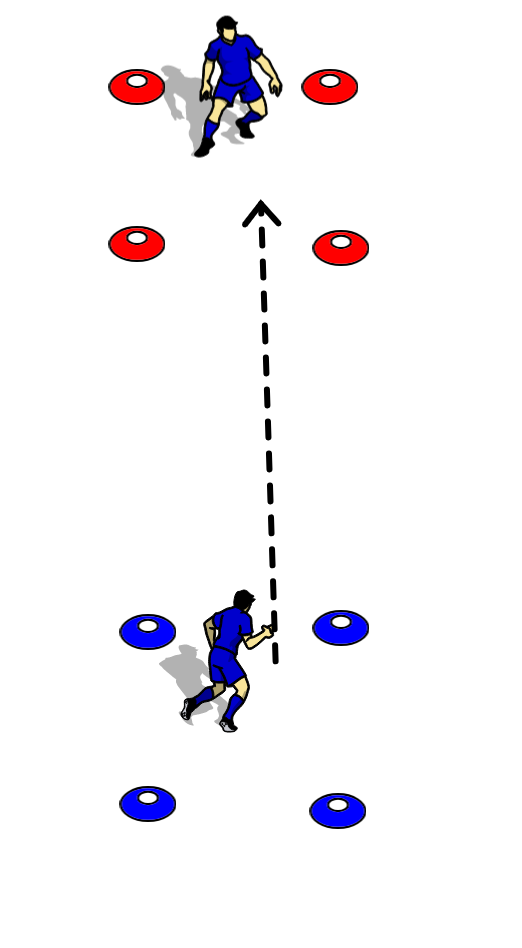
\includegraphics[width=.6\textwidth]{../img/Trimmed/Box_Passing_BW}
    \end{minipage}
    \hspace{0.05\linewidth}
    \begin{minipage}{.6\linewidth} % Left column and width
        \textbf{Drill Description:}

        \begin{enumerate}
        \setlength{\itemsep}{0pt}
        \setlength{\parskip}{0pt}
        \setlength{\parsep}{0pt}
        \item Two players stand in a 2 yard square box.  Boxes should be spaced about 5 yards apart.
        \item Players pass the ball to their partner in the 2 yard box.
        \item The partner tries to trap the ball within the box and pass it back.
        \item Alternate passing \& trapping foot half way through drill.
        \end{enumerate}

        \textbf{Coaching Points:}
        \begin{itemize}
        \setlength{\itemsep}{0pt}
        \setlength{\parskip}{0pt}
        \setlength{\parsep}{0pt}
        \item Focus on passing accurately with pace.
        \begin{itemize}
            \item Making a single step toward the ball.  This requires the ball to be one step in front of you.
            \item Hitting the center of the ball inside of your foot.
            \item Follow through.
        \end{itemize} 
        \item The goal is to trap the pass using a single touch.
        \item Stay on your toes at all times, this will keep you ready to move.  If you find it hard, focus on bouncing in place.
        \end{itemize}

    \end{minipage}
\end{minipage}

\end{oddBlock}